\chapter{Implementation}
\section{Web Application}
The program is taking the format of a web application with different musicality exercises on them. Users can pick and choose whatever exercises they would like to complete, which are grouped by category.
\subsection{Application flow}
	\subsubsection{Django web framework}
		\paragraph{Views}
		\paragraph{Models}
		Django interfaces with the database through Models. An example of this is the IntervalScore model below. This particular model stores all the information about a user's attempt at singing an interval in the interval training exercise.
		\begin{verbatim}
		class IntervalScore(models.Model):
   			interval = models.ForeignKey(Interval) 
    		timestamp = models.DateTimeField(auto_now_add=True)
    		score = models.FloatField();
		    user = models.PositiveIntegerField();
		    def __str__(self):
        		return " Score: " + str(self.score) + " for" + self.interval.name + " with user id: " + str(self.user)

		\end{verbatim}
		The interval field represents the interval that the user has attempted, the timestamp tells us when it was attempted, and the score field tells us the calculated score for that attempt (it will be explained how this metric is derived in "Measuring user ability")
		
\section{Pitch Detection}
\par Pitch detection is an important part of the exercises, and as such, robust pitch detection has been an important feature in the development of this program. 
\par Most existing pitch detection algorithms are based on real-time applications, i.e. where audio captured from a microphone is analysed and the pitch is displayed as a constantly updating function of the audio signal. This is useful for applications like guitar tuning, where you need near instant feedback, and you can be sure that the pitch you are inputting is fairly constant. 
\par With analysis of pitch in the human voice however, the problem is that even with well trained singers, the pitch of a note can vary quite considerable over a 2 second period, due to vibrato\footnote{Vibrato is the musical technique of intentionally oscillating the pitch of the note around a fixed point.}, or other causes that can be hard to pick up just by listening to yourself, so it is not always trivial to determine one pitch to summarise a sample of a single held note, and indeed, often not appropriate to do so if the singer cannot even stay on the same note for that short period of time, and wobbles around the note inconsistently.
\par It is with this in mind that I have developed a Segmented Pitch Detection Algorithm, that can accurately determine the pitch of a 2-3 second sample of singing.

\subsection{Segmented Pitch Detection Algorithm}
The principle of the Segmented Pitch Detection Algorithm is relatively simple: A given audio sample is split into several segments, pitch detection is run on each segment, and then the segments are analysed to calculate pitch. I have also employed several error detection/correction methods that are detailed below.
\begin{figure}
	\centering
	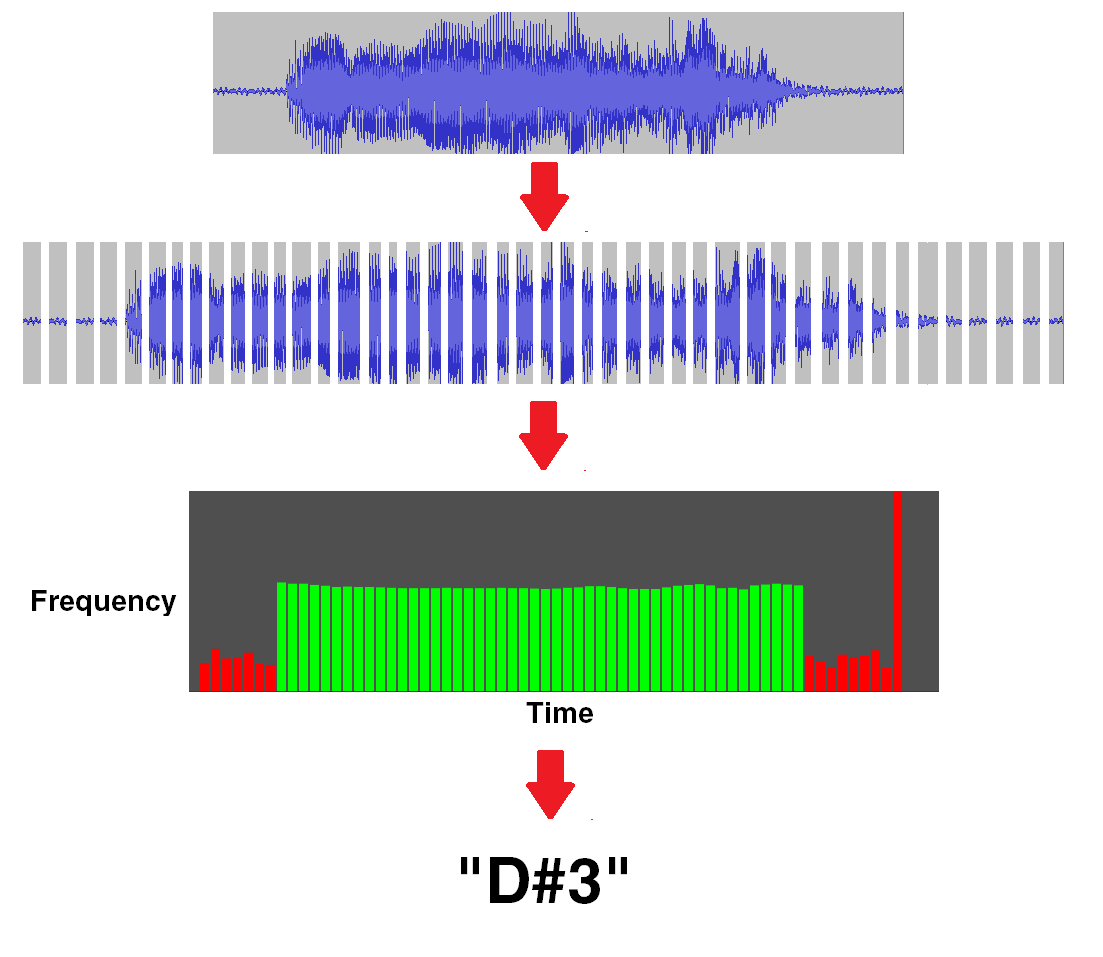
\includegraphics[scale=0.6]{segmented_autocorrelation.png}
	\caption{An illustration of how Segmented Autocorrelation works}
\end{figure}
\subsubsection{Choosing a segment size}
\par Most PC microphones sample audio at either 44,100Hz or 48,000Hz, as these ensure that the full 20KHz spectrum of human hearing can be recorded due to the Nyquist–Shannon sampling theorem (see Background section 2.5). For the sake of simplicity we will assume a sample rate of 48,000Hz for this report, though the program can handle either rate.
\par The human vocal range defined in section 2.4.2 was E2 - C6, which corresponds to a frequency range of ~80-1000hz\cite{scientificPitchTable}. To calculate the number of samples at either end of the range: 
 		 \[48000\div 96 = 600 \text{ samples}\] 
		 \[48000\div 1000 = 48 \text{ samples}\]
		
\par In order for our autocorrelation algorithm to work, it is  necessary to take a segment size at least twice that of the lowest frequency we wish to sample.
This is because in autocorrelation, we must compare the signal with an offset version of itself, and this score is maximal with an offset equal to the period of the signal. Therefore, in our example, if we use anything less than a 1200 sample size and are trying to detect a 96Hz signal, we won't even be able to autocorrelate on a full period. [DIAGRAM illustrating how you only compare half a period of you use a 900 sample segment] I have therefore decided to use 1200 as the segment size. Increasing this number results in a higher quality analysis per segment, but the trade-off is that segments per second decreases, meaning you are sacrificing granularity of change of pitch over time. [DIAGRAM of debug freqs graph at differing window sizes.

		
\subsubsection{Median Filtering}
Median filtering is a noise reduction process used when sharp spikes occur in a signal. It typically works using a sliding window algorithm, applying a median filter to all the elements in a grid.
\begin{figure}[h]	
	\centering	
	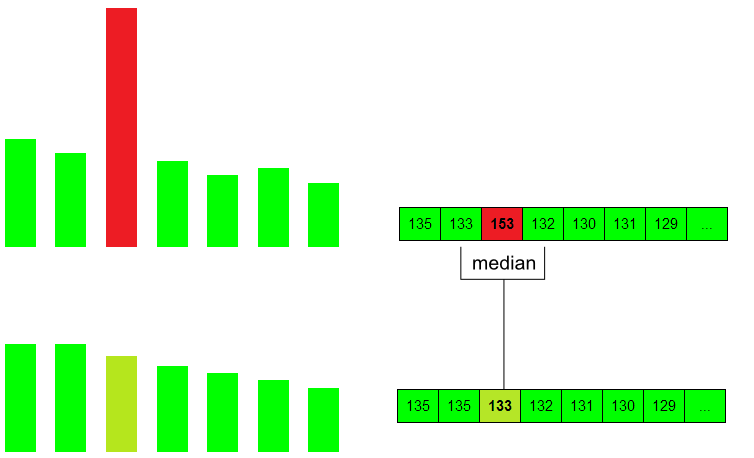
\includegraphics[scale=0.7]{median_demonstration.png}
	\caption{An example of median filtering with window size 3}
\end{figure}



\section{Measuring user ability}

User ability is measured through a level system. Every user has a level value assigned to each exercise they attempt, as well as for each category, and every user has an overall level also. Users with a high level will not have to start from the beginning when attempting new exercises. 

All users start at at level 1 when they sign up.

To increase their level, the user has to complete exercises correctly. As their level increases, the exercises adapt and get harder.

Measuring user ability is achieved by assigning a score to every \bsq{attempt} at a certain exercise. These scores are then processed by the server to determine:
	\begin{itemize}
		\item Whether the user should be levelled up.
		\item What questions it is best to ask them.
	\end{itemize}

\subsection{Interval training}

The scoring system for interval training is as follows:

\[\text{difference} = |P_\text{actual}- P_\text{target}|\]
\[\text{perfect\_score} = 0.1 \]
\[\text{distance\_from\_perfect} = \text{max}(\text{difference}-\text{perfect\_score},0)\]
\[\text{score} = \text{max}(1 - \text{distance\_from\_perfect},0)\]

Intuitively, this means that any interval attempt less than 0.1 semitones from the actual pitch is classed as a perfect score, and anything over 1.1 semitones away is classed as a zero,with values between those 0.1 and 1.1 semitones determined by linear interpolation.

\subsection{Note from chord}
\subsection{Beat reproduction}

\section{Adapting to user ability}
Discussion of the adaptive element of the program for different exercises.
\section{Exercises}

